\begin{note}All printed documents allowed. Send your code via the campus website (zip files if several files are to be sent).\end{note}

\section{Segmentation (13 points)}
% The principle of the adaptive threshold is to compare each pixel to a threshold that varies according the an average filter.
% 
% \begin{algorithm}[H]
% % \SetAlgoLined\DontPrintSemicolon
% %   \SetKwFunction{algo}{algo}
% \KwData{$in$ and $out$ are input and output images}
% \KwData{$h$ is the size of neighbordhood}
% \KwData{$t$ is a percentage value (between 0 and 1)}
% \SetKwFunction{func}{func}
% %   \SetKwProg{myalg}{Algorithm}{}{}
% %   \myalg{\algo{}}{
% %   \nl xxx\;
% %   \nl xxx\;
% %   \nl \proc{}\;
% %   \nl \KwRet\;}{}
% %   \setcounter{AlgoLine}{0}
%   \SetKwProg{myfunc}{function}{}{}
%   \myfunc{\func{in, out, h, t}}{
%   \nl $LA\leftarrow$ average filter of size $h$ of image $in$\;
%   \nl \ForEach{pixel $p$ of $in$}{
% 	\uIf{$in(p)\leq LA(p)*(1-t)$}{ $out(p)\leftarrow$0\;}
%     \Else{$out(p)\leftarrow$1\;}
% 	} 
%   \nl \KwRet $out$\;
% 	}
%   \caption{Algorithm of adaptive thresholding from Bradley.}
% \end{algorithm}

\begin{qbox}
 \begin{itemize}
  \item Segment the image.
 \end{itemize}

\end{qbox}

\begin{figure}[htbp]
\centering\caption{Test image}%
 \subfloat[Image to be segmented, from \cite{Bradley2007}.]{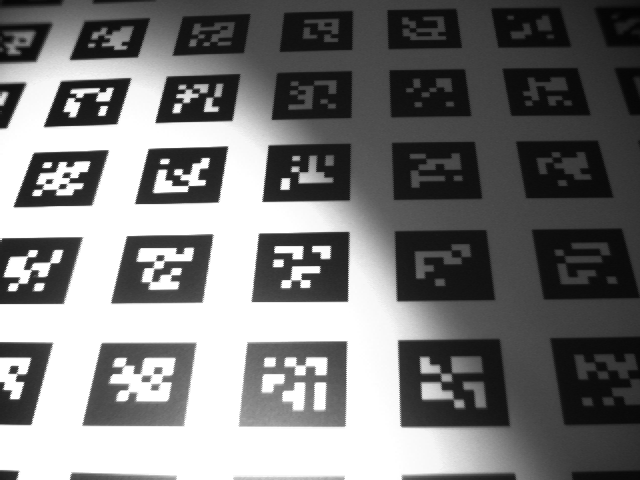
\includegraphics[width=5cm]{local_threshold.png}} \hspace{1cm}
 \subfloat[Segmented image]{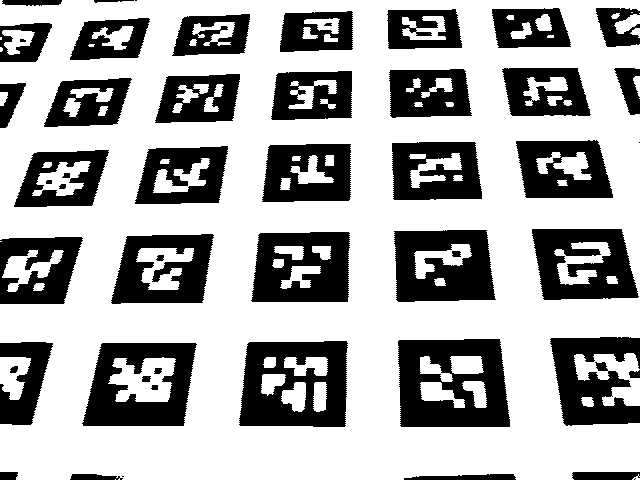
\includegraphics[width=5cm]{result_local_threshold.png}}
 \label{fig:test}
 \vspace*{-10pt}
\end{figure}

% \subsection{Correction proposition}
% Le premier réflexe est de réaliser un seuil global sur l'image. Cela ne fonctionne évidemment pas. Il faut donc se tourner vers un seuil local. Dans le cours sur la segmentation, une formule donne un seuil local, calculé dans une fenêtre $w$ autour du pixel selon la formule: $\mu_w +\alpha\sigma_w$ avec $\mu_w$ la moyenne dans la fenêtre, $\sigma_w$ l'écart-type des intensités dans $w$ et $\alpha$ un paramètre à déterminer. Une version proche est proposée ici:
% 
% \begin{matlab}
% function B=adaptiveThreshold(I, h, percent)
% % function adaptive thresholding, from bradley
% % I: image
% % h: size of neighborhood
% % percent: percentage of threshold (<=1)
% 
% B = zeros(size(I));
% LA = zeros(size(I));
% LA = filtre_moyenneur(I, h);
% for i=1:size(I,1)
%     for j=1:size(I,2)
%         if (I(i,j)<= LA(i,j)*(1-percent))
%             B(i,j) = 0;
%         else
%             B(i,j) = 255;
%         end
%     end
% end
% %figure
% %imshow(B,[])
% 
%     function M = filtre_moyenneur(I, h)
%         H = fspecial('average', h);
%         M = imfilter(I, H);
%     end
% 
% 
% end
% \end{matlab}

\section{Integral image (7 points)}
If the original image is denoted $f$, the integral image $I$ is defined by the following equation, for all pixels of coordinates $(x,y)$:
$$I(x,y)=f(x,y)+I(x-1,y)+I(x,y-1)-I(x-1,y-1)$$
	
	\begin{qbox}
	 \begin{itemize}
	  \item Code a function that computes this integral image. The prototype of this function must be \minline{function II=int_image(I)}.

	  \item Code a function that computes the local average of the image $f$. Notice that: 
	  \begin{equation*}
	  \begin{aligned}\sum_{x=x_1}^{x_2}\sum_{y=y_1}^{y_2}f(x,y) &= I(x_2,y_2)-I(x_2,y_1-1)\\
	  &-I(x_1-1,y_2)+I(x_1-1, y_1-1)
	  \end{aligned}
	  \end{equation*}

	  \item Compare it to a mean filter.
	 \end{itemize}

	\end{qbox}
	
	\begin{mcomment}
	 \begin{mremark}
	  The mean filter can be coded with the \matlabregistered{} functions \minline{imfilter} and \minline{fspecial} (result and computation time).
	 \end{mremark}

	\end{mcomment}

	
% \subsection{Proposition de correction}
% Une chose évidente, que personne n'a faite, aurait été de chercher dans l'aide de \matlabregistered{} une fonction de calcul d'une image intégrale: \minline{integralImage}. 
% 
% Le nom de cette fonction aurait pu vous mettre sur une piste: l'intégrale, ou en discret la somme cumulée, de toutes les valeurs en partant du haut à gauche et en suivant un rectangle. La fonction se résume basiquement à faire:
% \begin{matlab}
% cumsum(cumsum(I,2))
% \end{matlab}
% 
% Pour détailler le calcul, voici ma version qui donne une image intégrale légèrement plus grande que l'image d'origine:
% \begin{matlab}
% function II=int_image(I)
% % function of computation of integral image
% I2 =  zeros(size(I)+1);
% II = I2;
% I2(2:end, 2:end) = I;
% 
% for i=2:size(I2,1)
%     for j=2:size(I2,2)
%         II(i,j)=I2(i,j)+II(i-1,j)+II(i,j-1)-II(i-1,j-1);
%     end
% end
% 
% % test the difference with the \matlabregistered{} equivalent function
% %test(II, integralImage(I));
% 
%     function test(I1, I2)
%         disp('test difference:')
%         d = sum(sum(abs(I2-I1)))
%     end
% end
% \end{matlab}
% 
% Pour calculer la moyenne locale dans le rectangle $(x_1,y_1), (x_2,y_2)$, la formule revient à:
% $$\frac{1}{N}(II(x_1,y_1)+II(x_2,y_2) - II(x_1,y_2) - II(x_2,y_1))$$
